\documentclass[12pt,letterpaper]{article}

\usepackage[spanish,es-tabla,es-nodecimaldot]{babel}
\usepackage{amsmath}
\usepackage[utf8]{inputenc}
\usepackage[T1]{fontenc}
\usepackage{lmodern}
\usepackage{graphicx}
\usepackage{listings}
\usepackage{anysize} 
\usepackage{fancyhdr}
\usepackage{amsmath}
\usepackage{pdfpages}
\usepackage{graphics}
\usepackage{capt-of}
\usepackage{tabularx}
\usepackage{booktabs}
\usepackage[colorlinks=true,plainpages=true,citecolor=blue,linkcolor=blue]{hyperref}

\usepackage{xcolor}

\definecolor{mGreen}{rgb}{0,0.6,0}
\definecolor{mGray}{rgb}{0.5,0.5,0.5}
\definecolor{mPurple}{rgb}{0.58,0,0.82}
\definecolor{backgroundColour}{rgb}{0.95,0.95,0.92}

\marginsize{2cm}{2cm}{2cm}{2cm}
\pagestyle{fancy}
\fancyhf{Teoría de la Información}
\fancyhead[L]{\footnotesize UPIITA-IPN} 
\fancyhead[R]{\footnotesize 2TM4} 
\fancyfoot[R]{\footnotesize Práctica 5}
\fancyfoot[C]{\thepage}
\fancyfoot[L]{\footnotesize Reporte} 
\renewcommand{\footrulewidth}{0.4pt}
\renewcommand{\spanishtablename}{Tabla}
\renewcommand{\labelitemii}{$\star$}
\lstdefinestyle{CStyle}{
    backgroundcolor=\color{backgroundColour},   
    commentstyle=\color{mGreen},
    keywordstyle=\color{magenta},
    numberstyle=\tiny\color{mGray},
    stringstyle=\color{mPurple},
    basicstyle=\footnotesize,
    breakatwhitespace=false,         
    breaklines=true,                 
    captionpos=b,                    
    keepspaces=true,                 
    numbers=left,                    
    numbersep=5pt,                  
    showspaces=false,                
    showstringspaces=false,
    showtabs=false,                  
    tabsize=2,
    language=C
}

\graphicspath{ {C:/Users/Anselmo-PC/Documents/GitHub/upiita-RedesTelecomunicaciones/MemoriaTecnica/imagenes} }

\begin{document}

\includepdf[pages={1}]{portada}
\newpage
\tableofcontents
\listoffigures

\newpage
\section{Objetivo}
Implementación en hardware de un codificador de canal de bloque mediante la utilizacion 
de dispositivos lógicos programables.

\section{Descripción}
A partir de una matriz generadora perteneciente a un CBS(n, k), se implementrán en dispositivo 
programable tanto la parte codificadora (coder) como la parte decodificadora (decoder) de dicho
codificador, de acuerdo con el siguiente diagrama.
\begin{figure}[ht]
    \centering
    
\includegraphics[width=1\textwidth]{d0.png}
    \caption{Daigrama a bloques general del codificador a implementar.}
\end{figure}

\newpage
\section{Diagrama de circuito de implementación}
\begin{figure}[ht]
    \centering
    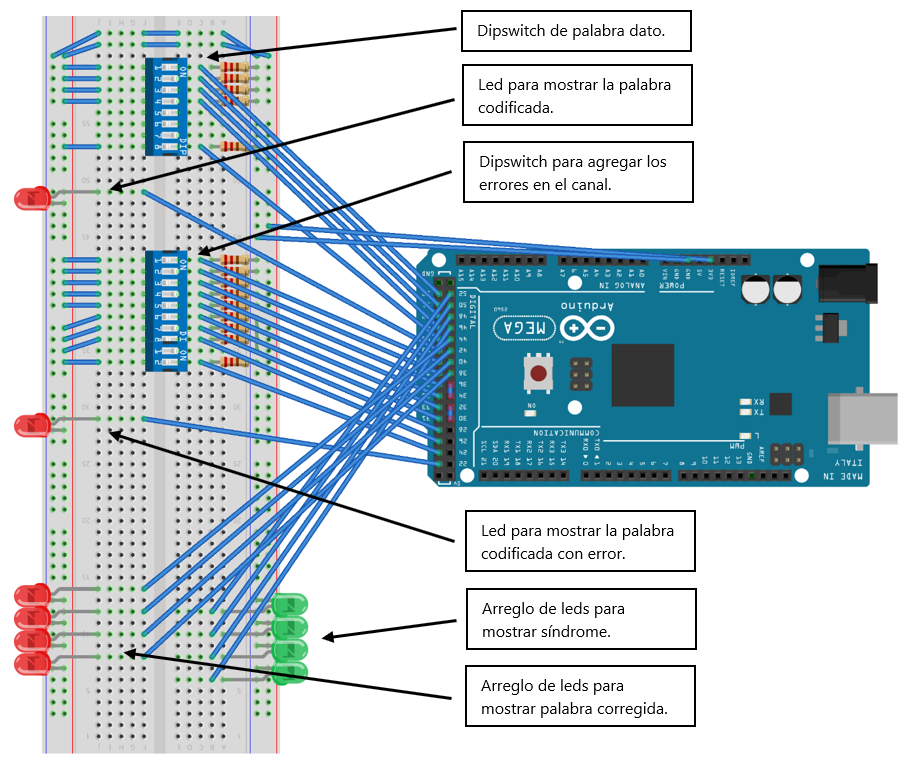
\includegraphics[width=.75\textwidth]{circ.png}
    \caption{Circuito implementado.}
\end{figure}

\subsection{Timers utilizados}
\begin{figure}[ht]
    \centering
    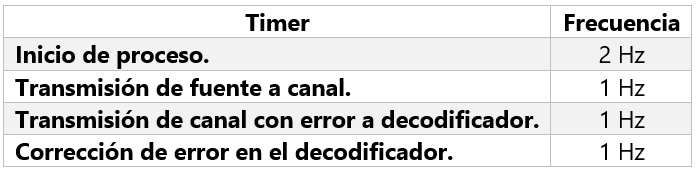
\includegraphics[width=.6\textwidth]{reloj.png}
    \caption{Timers.}
\end{figure}

\newpage
\section{Código}
\begin{lstlisting}[style=CStyle]
// Libreria para operaciones logicas
#include <iso646.h>
// Pins para palabra dato, control de fuente y muestra
// de transmision
#define D1 53
#define D2 51
#define D3 49
#define D4 47

#define CD 45

#define C1 43
// Pins para error, control de canal y muestra
// de transmision
#define E1 41
#define E2 39
#define E3 37
#define E4 35
#define E5 33
#define E6 31
#define E7 29
#define E8 27

#define CE 25

#define C2 23
// Pins para sindrome
#define S1 52
#define S2 50
#define S3 48
#define S4 46
// Pins para palabra corregida
#define COR1 44
#define COR2 42
#define COR3 40
#define COR4 38
// Pins para canal
#define CCOUT1 36
#define CCIN1 34
// Pins para canal
#define CCOUT2 32
#define CCIN2 30

// Variables globales para codificacion  y decodficacion
int d1, d2, d3, d4, cd, c1, c2;
int ce[8]{ 0,0,0,0,0,0,0,0 };
int error[8]{ 0,0,0,0,0,0,0,0 };
int r[8]{ 0,0,0,0,0,0,0,0 };
int sindrome[4]{ 0,0,0,0 };
int cr[8]{ 0,0,0,0,0,0,0,0 };

// Prototipo de funciones
void ReadPins();
void TransmisionCanalError(int codidgo[8]);
void PatronError();
void AgregaError();
void ObtieneSindrome(int error[8]);
void TransmisionErrorDecoder(int codidgo[8]);
void DecodificaPalabra();

// Funcion de inicio
void setup()
{
	// Asignar un modo a los pines a utilizar
	ReadPins();
	Serial.begin(9600);
	Serial.println("Puerto abierto");
}

// Funcion de proceso principal
void loop()
{
	// Condiciones iniciales
	delay(2000);
	digitalWrite(COR1, 0);
	digitalWrite(COR2, 0);
	digitalWrite(COR3, 0);
	digitalWrite(COR4, 0);
	digitalWrite(S1, 0);
	digitalWrite(S2, 0);
	digitalWrite(S3, 0);
	digitalWrite(S4, 0);

	// Control de fuente
	cd = digitalRead(CD);
	while (cd == 0)
		cd = digitalRead(CD); // Permitir transmision

	// Lectura de palabra dato
	int codigo[8]{ 0,0,0,0,0,0,0,0 };
	d1 = digitalRead(D1);
	d2 = digitalRead(D2);
	d3 = digitalRead(D3);
	d4 = digitalRead(D4);

	// Generacion de palabra codigo
	codigo[0] = d2 ^ d3 ^ d4;
	codigo[1] = d1 ^ d2 ^ d3;
	codigo[2] = d1 ^ d2 ^ d4;
	codigo[3] = d1 ^ d3 ^ d4;
	codigo[4] = d1;
	codigo[5] = d2;
	codigo[6] = d3;
	codigo[7] = d4;

	// Se inicia la transmision de la fuente 
	// al canal
	TransmisionCanalError(codigo);

	// Se prepara el error en el canal y se 
	// controla la transmision
	if (digitalRead(CE))
	{
		// Leer los errores a agregar
		PatronError();
		// Agrega el error a la palabra
		AgregaError();
		// Se transmite la palabra codigo con error al 
		// decoder
		TransmisionErrorDecoder(ce);
		// Se obtiene el sindrome a partir del error 
		// del canal
		ObtieneSindrome(error);
		// Se corrige la palabra recibida
		DecodificaPalabra();
	}
}

// Asignacion de modo en los pines
void ReadPins()
{
	pinMode(D1, INPUT);
	pinMode(D2, INPUT);
	pinMode(D3, INPUT);
	pinMode(D4, INPUT);

	pinMode(CD, INPUT);

	pinMode(C1, OUTPUT);

	pinMode(E1, INPUT);
	pinMode(E2, INPUT);
	pinMode(E3, INPUT);
	pinMode(E4, INPUT);
	pinMode(E5, INPUT);
	pinMode(E6, INPUT);
	pinMode(E7, INPUT);
	pinMode(E8, INPUT);

	pinMode(CE, INPUT);

	pinMode(C2, OUTPUT);

	pinMode(S1, OUTPUT);
	pinMode(S2, OUTPUT);
	pinMode(S3, OUTPUT);
	pinMode(S4, OUTPUT);

	pinMode(COR1, OUTPUT);
	pinMode(COR2, OUTPUT);
	pinMode(COR3, OUTPUT);
	pinMode(COR4, OUTPUT);

	pinMode(CCOUT1, OUTPUT);
	pinMode(CCOUT2, OUTPUT);

	pinMode(CCIN1, INPUT);
	pinMode(CCIN2, INPUT);
}

void TransmisionCanalError(int codidgo[8])
{
	Serial.println("Transmision fuente -> canal");
	// Se inicia la transmision serial
	for (auto i = 0; i < 8; ++i)
	{
		// Se transmite al canal
		digitalWrite(CCOUT1, codidgo[i]);
		// Se lee el dato transmitido al canal
		ce[i] = digitalRead(CCIN1);
		// Se muestra el dato recibido
		digitalWrite(C1, ce[i]);
		Serial.print(ce[i]);
		// Timer
		delay(1000);
	}
	Serial.println();
	Serial.println("Transmision terminada");
	// Se liberan recursos
	digitalWrite(C1, 0);
}

void PatronError()
{
	// Se leen los errores a agregar a
	// la palabra codigo
	error[0] = digitalRead(E1);
	error[1] = digitalRead(E2);
	error[2] = digitalRead(E3);
	error[3] = digitalRead(E4);
	error[4] = digitalRead(E5);
	error[5] = digitalRead(E6);
	error[6] = digitalRead(E7);
	error[7] = digitalRead(E8);
	Serial.println("Patron error");
	/*for (int i = 0; i < 8; ++i)
		Serial.print(error[i]);
	Serial.println();*/
}

void AgregaError()
{
	// Se busca donde fue configurado el error
	// y se agrega a la palabra codigo
	if (error[0]) ce[0] = ce[0] xor 1;
	if (error[1]) ce[1] = ce[1] xor 1;
	if (error[2]) ce[2] = ce[2] xor 1;
	if (error[3]) ce[3] = ce[3] xor 1;
	if (error[4]) ce[4] = ce[4] xor 1;
	if (error[5]) ce[5] = ce[5] xor 1;
	if (error[6]) ce[6] = ce[6] xor 1;
	if (error[7]) ce[7] = ce[7] xor 1;
	/*Serial.println("Codigo con error");
	for (int i = 0; i < 8; ++i)
		Serial.print(ce[i]);
	Serial.println();*/
}

void ObtieneSindrome(int error[8])
{
	// Si el canal dejo de transmitir se cancela la 
	// operacion
	if (!cr[0] && !cr[1] && !cr[2] && !cr[3] && !cr[4] && !cr[5] &&
		!cr[6]) return;

	// Se calcula el sindrome con base en la ecuaciones 
	// obtenidas
	sindrome[0] = error[0] ^ error[5] ^ error[6] ^ error[7];
	sindrome[1] = error[1] ^ error[4] ^ error[5] ^ error[6];
	sindrome[2] = error[2] ^ error[4] ^ error[5] ^ error[7];
	sindrome[3] = error[3] ^ error[4] ^ error[6] ^ error[7];

	// Se muestra el sindrome en el arreglo de leds asignados
	// en el circuito
	digitalWrite(S1, sindrome[0]);
	digitalWrite(S2, sindrome[1]);
	digitalWrite(S3, sindrome[2]);
	digitalWrite(S4, sindrome[3]);

	/*Serial.println("Sindrome");
	for (int i = 0; i < 4; ++i)
		Serial.print(sindrome[i]);
	Serial.println();*/
}

void TransmisionErrorDecoder(int codidgo[8])
{
	// Se inicia la transmision serial
	Serial.println("Transmision error -> decoder");
	for (auto i = 0; i < 8; ++i)
	{
		// Se transmite al canal
		digitalWrite(CCOUT2, codidgo[i]);
		// Se lee el dato transmitido al canal
		Serial.print(digitalRead(CCIN2));
		// Se muestra el dato recibido
		cr[i] = digitalRead(CCIN2);
		digitalWrite(C2, cr[i]);
		// Timer
		delay(1000);
	}
	Serial.println();
	Serial.println("Transmision terminada");
	// Se liberan recursos
	digitalWrite(C2, 0);
}

void DecodificaPalabra()
{
	// Si el sindrome es 0000, significa se interrumpio la 
	// transmision o no se ha transmitido algo, por lo que se cancela 
	// la funcnion
	if (!sindrome[0] && !sindrome[1] && !sindrome[2] && !sindrome[3])
		return;

	// Con base la matriz H transouesta se verifican la siguientes condiciones 
	// para corregir errores simples y dobles
	Serial.println("Corrigiendo errror");
	if (sindrome[0] && !sindrome[1] && !sindrome[2] && !sindrome[3]) //1000
	{
		cr[0] = cr[0] xor 1;
	}
	else if (!sindrome[0] && sindrome[1] && !sindrome[2] && !sindrome[3]) //0100
	{
		cr[1] = cr[1] xor 1;
	}
	else if (!sindrome[0] && !sindrome[1] && sindrome[2] && !sindrome[3]) //0010
	{
		cr[2] = cr[2] xor 1;
	}
	else if (!sindrome[0] && !sindrome[1] && !sindrome[2] && sindrome[3]) //0001
	{
		cr[3] = cr[3] xor 1;
	}
	else if (!sindrome[0] && sindrome[1] && sindrome[2] && sindrome[3]) //0111
	{
		cr[4] = cr[4] xor 1;
	}
	else if (sindrome[0] && sindrome[1] && sindrome[2] && !sindrome[3]) //1110
	{
		cr[5] = cr[5] xor 1;
	}
	else if (sindrome[0] && sindrome[1] && !sindrome[2] && sindrome[3]) //1101
	{
		cr[6] = cr[6] xor 1;
	}
	else if (sindrome[0] && !sindrome[1] && sindrome[2] && sindrome[3]) //1011
	{
		cr[7] = cr[7] xor 1;
	}
	else if (!sindrome[0] && sindrome[1] && !sindrome[2] && sindrome[3]) //0101 doble 2,4 
	{
		cr[1] = cr[1] xor 1;
		cr[3] = cr[3] xor 1;
	}
	else if (sindrome[0] && !sindrome[1] && sindrome[2] && !sindrome[3]) //1010 doble 1,3
	{
		cr[0] = cr[0] xor 1;
		cr[2] = cr[2] xor 1;
	}

	for (auto i = 4; i < 8; i++)
	{
		Serial.print(cr[i]);
	}

	// Se muestra la palabra corregida en el arrgle de 
	// leds asignados
	digitalWrite(COR1, cr[4]);
	digitalWrite(COR2, cr[5]);
	digitalWrite(COR3, cr[6]);
	digitalWrite(COR4, cr[7]);
	Serial.println("");
	// Timer
	delay(1000);
}
\end{lstlisting}

\section{Circuito lógico}
\subsection{Coder}
A partir de la matriz generadora G y la siguiente ecuación se pueden obtener la palabras código.
\begin{equation}
    \vec{c}=\vec{d}G
\end{equation}
Donde:
\begin{itemize}
    \item \textbf{$\vec{c}$: } palabra código.
    \item \textbf{$\vec{d}$: } palabra doto.
    \item \textbf{G: } matriz generadora.
\end{itemize}
La matriz generadora es la siguiente:
\[
G
=
\begin{bmatrix} 
    0 & 1 & 1 & 1 & 1 & 0 & 0 & 0 \\
    1 & 1 & 1 & 0 & 0 & 1 & 0 & 0 \\
    1 & 1 & 0 & 1 & 0 & 0 & 1 & 0 \\
    1 & 1 & 1 & 1 & 0 & 0 & 0 & 1 \\
    \end{bmatrix}
\]
El vector de la palabra dato es:
\begin{equation}
    \vec{d}=[d_1 \ d_2 \ d_3 \ d_4]
\end{equation}
Realizando la operación se podrán obtener los diferentes valores del vector $\vec{c}$.
Las ecuaciones resultantes de esta operación son las siguientes.
$$c_1=d_2 \bigoplus d_3 \bigoplus d_4$$
$$c_2=d_1 \bigoplus d_2 \bigoplus d_3$$
$$c_3=d_1 \bigoplus d_2 \bigoplus d_4$$
$$c_4=d_1 \bigoplus d_3 \bigoplus d_4$$
$$c_5=d_1$$
$$c_6=d_2$$
$$c_7=d_3$$
$$c_8=d_4$$

Y la palabra código resultante es:
\begin{equation}
    \vec{c}=[c_1 \ c_2 \ c_3 \ c_4 c_5 \ c_6 \ c_7 \ c_8]
\end{equation}

\newpage
\subsubsection{Circuito lógico}
\begin{figure}[ht]
    \centering
    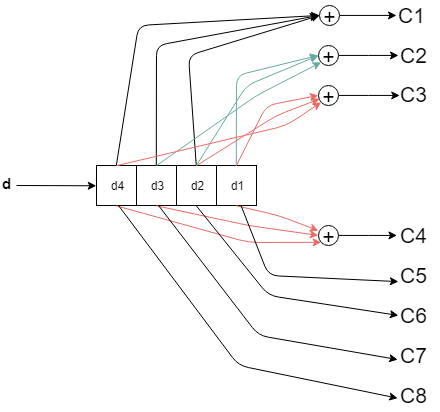
\includegraphics[width=.8\textwidth]{ccode.png}
    \caption{Circuito lógico codificador.}
\end{figure}

\newpage
\subsection{Decoder}
Para el proceso de corrección y decodficacion se debe de ontener la matriz \textbf{H}.
\begin{equation}
    H=[I P^T]
\end{equation}
Para obtener la ecuaciones del Síndrome se cálcula H transpuesta.
\[
H^T
=
\begin{bmatrix} 
    1 & 0 & 0 & 0 \\
    0 & 1 & 0 & 0 \\
    0 & 0 & 1 & 0 \\
    0 & 0 & 0 & 1 \\
    0 & 1 & 1 & 1 \\
    1 & 1 & 1 & 0 \\
    1 & 1 & 0 & 1 \\
    1 & 1 & 1 & 1 \\
\end{bmatrix}
\]
Las ecuaciones del Síndrome son:
$$s_1=r_1+r_6+r_7+r_8$$
$$s_2=r_2+r_5+r_6+r_7$$
$$s_3=r_3+r_5+r_6+r_8$$
$$s_4=r_4+r_5+r_7+r_8$$

\subsubsection{Circuito lógico síndrome}
\begin{figure}[ht]
    \centering
    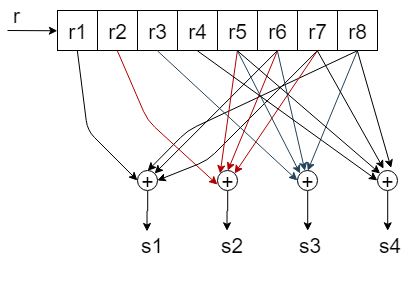
\includegraphics[width=.6\textwidth]{sind.png}
    \caption{Circuito lógico síndrome.}
\end{figure}

\newpage
Con ayuda de la misma matriz se pueden obtener las ecuaciones de error que ayudarán para 
la corrección de errores.
\\ \\
Errores simples.
$$e_1=s_1+\neg s_2+\neg s_3+\neg s_4$$
$$e_2=\neg s_1+s_2+\neg s_3+\neg s_4$$
$$e_3=\neg s_1+\neg s_2+s_3+\neg s_4$$
$$e_4=\neg s_1+\neg s_2+\neg s_3+s_4$$
$$e_5=\neg s_1+s_2+s_3+s_4$$
$$e_6=s_1+s_2+s_3+\neg s_4$$
$$e_7=s_1+s_2+\neg s_3+s_4$$
$$e_8=s_1+\neg s_2+s_3+s_4$$

Errores dobles.
$$e_{1,3}=s_1+\neg s_2+s_3+\neg s_4$$
$$e_{2,4}=\neg s_1+s_2+\neg s_3+s_4$$

\newpage
\subsubsection{Circuito lógico decodificador}
\begin{figure}[ht]
    \centering
    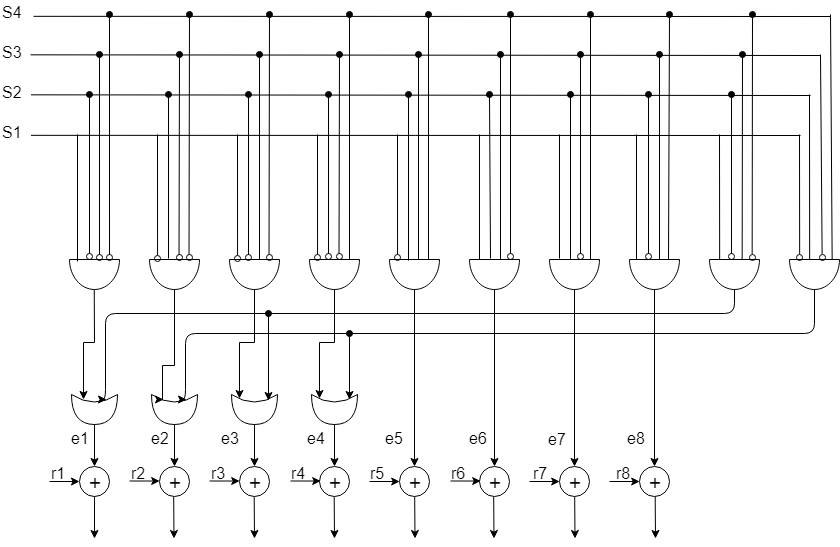
\includegraphics[angle=90,width=.58\textwidth]{decod.png}
    \caption{Circuito lógico decodificador.}
\end{figure}

\newpage
\section{Palabras dato y codigo}
\begin{figure}[ht]
    \centering
    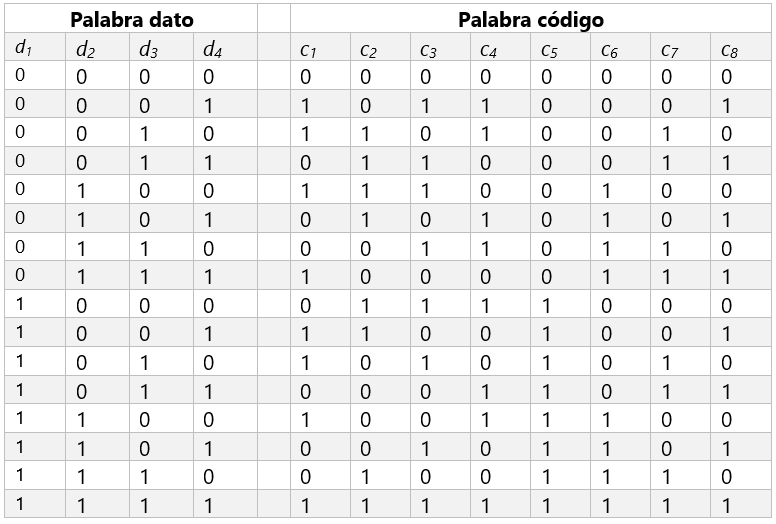
\includegraphics[width=1\textwidth]{pc.png}
    \caption{Palabras dato y codigo.}
\end{figure}

\newpage
\section{Síndrome vs patrón de error}
\begin{figure}[ht]
    \centering
    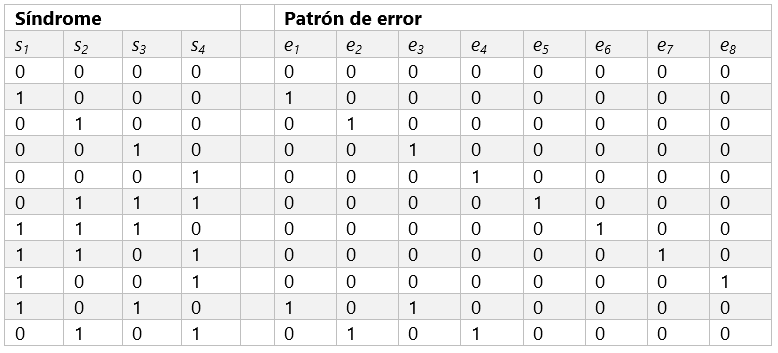
\includegraphics[width=1\textwidth]{sp.png}
    \caption{Síndrome vs patrón de error.}
\end{figure}

\newpage
\section{Resultados simulación}
La simulación fue realizada con ayuda del progrma Proteus y la librería simulino. Estas 
herramientas permiten ejecutar el código realizado en un arduino virtual.
\begin{figure}[ht]
    \centering
    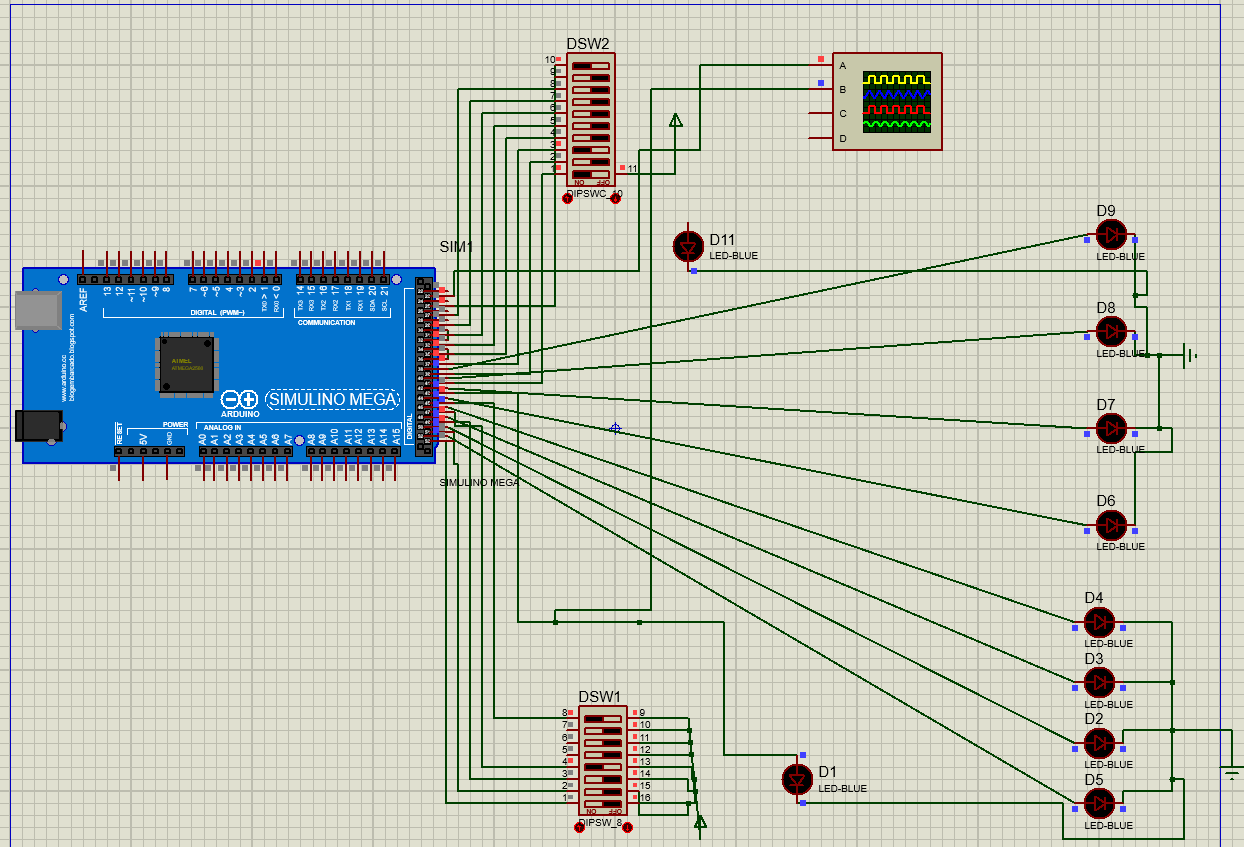
\includegraphics[width=1\textwidth]{simu0.png}
    \caption{Esquema de simulación.}
\end{figure}
\\
Para la simulación se utilzo la palabra dato \textbf{1010}, lo que da como resulatdo la palabra 
código \textbf{10101010}. Posteriomente se le agrego un error doble en las posiciones 2, 4. 
Agregando estos errores la palabra resultante con error es \textbf{11111010}.

\newpage
Como se muestra en la siguiente imagen, en el canal \textbf{A} se tiene la palabra codificada y el 
canal \textbf{B} la palabra codificada con error.
\begin{figure}[ht]
    \centering
    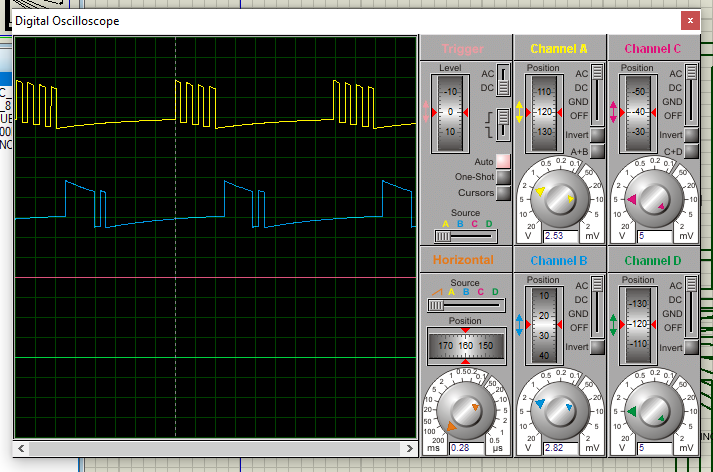
\includegraphics[width=1\textwidth]{simu1.png}
    \caption{Pulsos generados de la palabra código y la palabra código con error.}
\end{figure}
\newpage
En la última imagen de esta sección se muestra las palabra código, el síndrome y la palabra 
dato recuperada después de corregir el error y decodificarla, que fue \textbf{1010}.
\begin{figure}[ht]
    \centering
    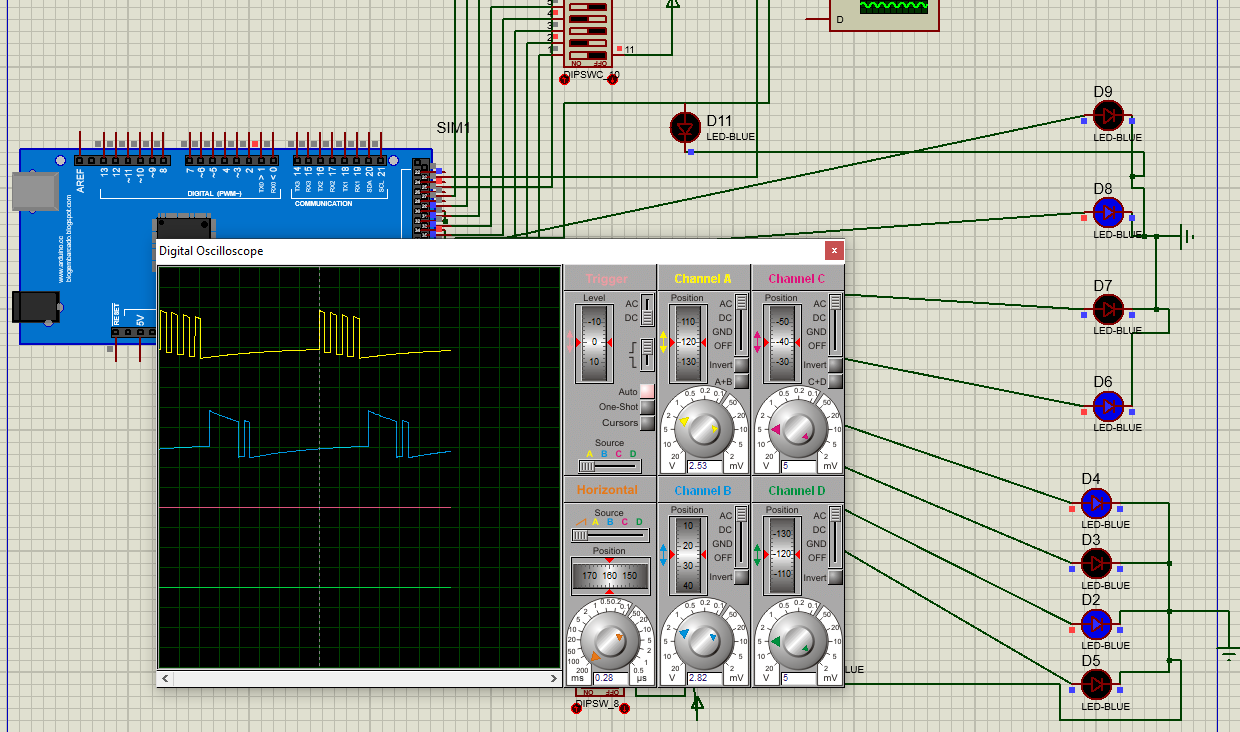
\includegraphics[width=1\textwidth]{simu2.png}
	\caption{Pulsos generados de la palabra código, palabra código con error, síndrome y 
	palabra dato.}
\end{figure}

\newpage
\section{Listado de asignación de terminales}
\begin{figure}[ht]
    \centering
    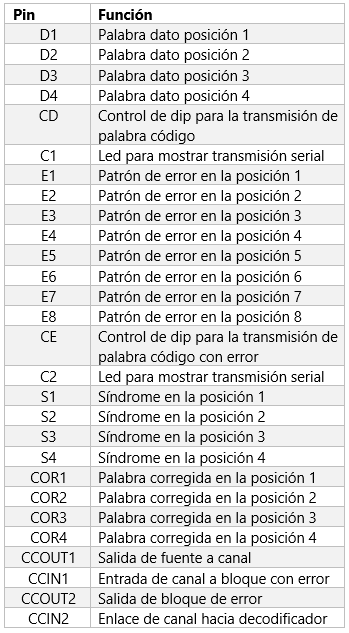
\includegraphics[width=.49\textwidth]{pines.png}
    \caption{Terminales.}
\end{figure}

\newpage
\section{Diagramas de flujo}
\begin{figure}[ht]
    \centering
    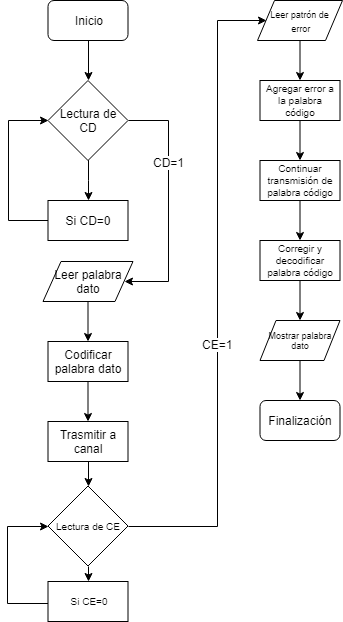
\includegraphics[width=.48\textwidth]{flujo0.png}
    \caption{Diagrama principal.}
\end{figure}

\newpage
\subsection{Codificador}
\begin{figure}[ht]
    \centering
    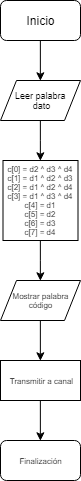
\includegraphics[width=.15\textwidth]{flujo1.png}
    \caption{Codificador.}
\end{figure}

\newpage
\subsection{Decodificador}
\begin{figure}[ht]
    \centering
    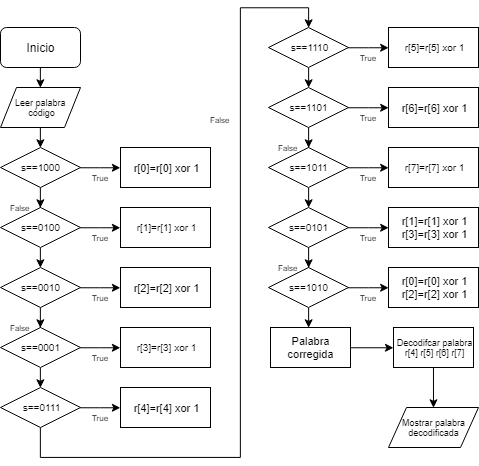
\includegraphics[width=.9\textwidth]{flujo2.png}
    \caption{Decodificador.}
\end{figure}

\newpage
\subsection{Utilización de dispositivo}
De acuerdo con información por el IDE de arduino, la utilización es la siguiente.
\begin{figure}[ht]
    \centering
    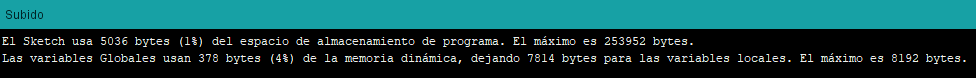
\includegraphics[width=1\textwidth]{uti.png}
    \caption{Utilización.}
\end{figure}

\section{Conclusiones}
Al comienzo de la realización de la práctica fue necesario empezar con el análisis del caso particular 
asignado. Este análisis permitió conocer las ecuaciones que debían ser implementadas para el desarrollo 
de la práctica. La matriz generadora asignada fue particular, ya que el componente de paridad se 
encontraba invertido, lo que al inicio fue algo confuso. Pero después de investigar acerca de esta 
característica, se encontró la solución, la cual no distaba mucho de lo aprendido en clase.
\\ \\
Aparte del punto mencionado anteriormente, el análisis para encontrar las ecuaciones para la 
codificación, para obtener el síndrome y las ecuaciones de error, se desarrolló normalmente. 
Cabe mencionar que para este caso se debía de contemplar dos pares de errores dobles en las posiciones 
[1,3] y [2,4]. 
\\ \\
En la implementación se requirió que la comunicación entre los bloques del codificador, el canal 
y el decodificador fueran en serie, lo que supuso una dificultad. Para sortear esto surgieron dos 
ideas, controlar la transmisión del codificador y del canal o sincronizar los datos transmitidos. 
Se optó por controlar la transmisión del codificador y del canal, ya que permitía tener un mejor 
control de los componentes y eventos dentro del programa. La comunicación serial en este caso fue 
realizada mediante dos puentes dentro del mismo Arduino y con un pin extra de salida para mostrar 
los datos transmitidos.
\\ \\
En la etapa de pruebas se introdujeron las combinaciones para una palabra dato de 4 bits. 
Así mismo, se probaron los errores simples en todas las posiciones disponibles y los pares de 
errores dobles. Posteriormente se probaron errores dobles en diferentes posiciones e incluso errores 
triples. Como resultado de esta última etapa de pruebas para el decodificador, mientras que realizaba 
algo, no necesariamente era correcto. Esto debido a que fue diseñado para casos específicos de errores 
dobles con la capacidad de corregir errores simples. En algunos casos podría decirse que corrigió 
correctamente, pero esta respuesta debió clasificarse como falso positivo, ya que la entrada no era 
la correcta.
\\ \\
Con la realización de esta última práctica se entendió mejor la manera en que la corrección 
de errores es implementada en un sistema de comunicación. Es importante señalar que la etapa de 
análisis es fundamental y debe de revisarse y comprobarse en busca de errores que puedan afectar 
en la implementación. También se debe de contemplar las limitaciones que el diseño y la implantación 
tenga, para dejar claro lo que es capaz de realizar.

\end{document}